\documentclass[usenames,dvipsnames,notes,11pt,aspectratio=169,hyperref={colorlinks=true, linkcolor=blue}]{beamer}
\usepackage{ifthen}
\usepackage{xcolor}
\usepackage{pgfplots}
\usepackage{amsmath}
\usepackage{centernot}
\usepackage{pifont}
\usepackage{tabularx}
\usepackage{makecell}
\usepackage{cuted}
\usepackage{booktabs}
\usepackage{array}
\usepackage{textcomp}
\usepackage{setspace}
\usepackage{xspace}
\usepackage{subcaption}
\usepackage{mdframed}
\usepackage{tikz}
\usepackage{pdfcomment}
%\newcommand{\pdfnote}[1]{\marginnote{\pdfcomment[icon=note]{#1}}}
\newcommand{\pdfnote}[1]{}

\usepackage{pgfpages}
%\setbeameroption{show notes on second screen}


\input ../beamer-style
\input ../std-macros
\input ../macros

\newcommand{\pt}{\partial}

\AtBeginSection[]
{
    \begin{frame}
        \frametitle{Table of Contents}
        \tableofcontents[currentsection]
    \end{frame}
}
\parskip=10pt

\title[DS-GA.1011]{Aligning Language Models II}
\author[He He]{He He
}
\institute[NYU]{
    
\includegraphics[height=1cm]{../figures/nyu-logo}\\
}
\date{November 29, 2023}

\begin{document}
\begin{frame}
\titlepage
\end{frame}

\begin{frame}
    {Logistics}
    Next week: online guest lecture by Victoria Lin \url{http://victorialin.net}
        \begin{figure}
            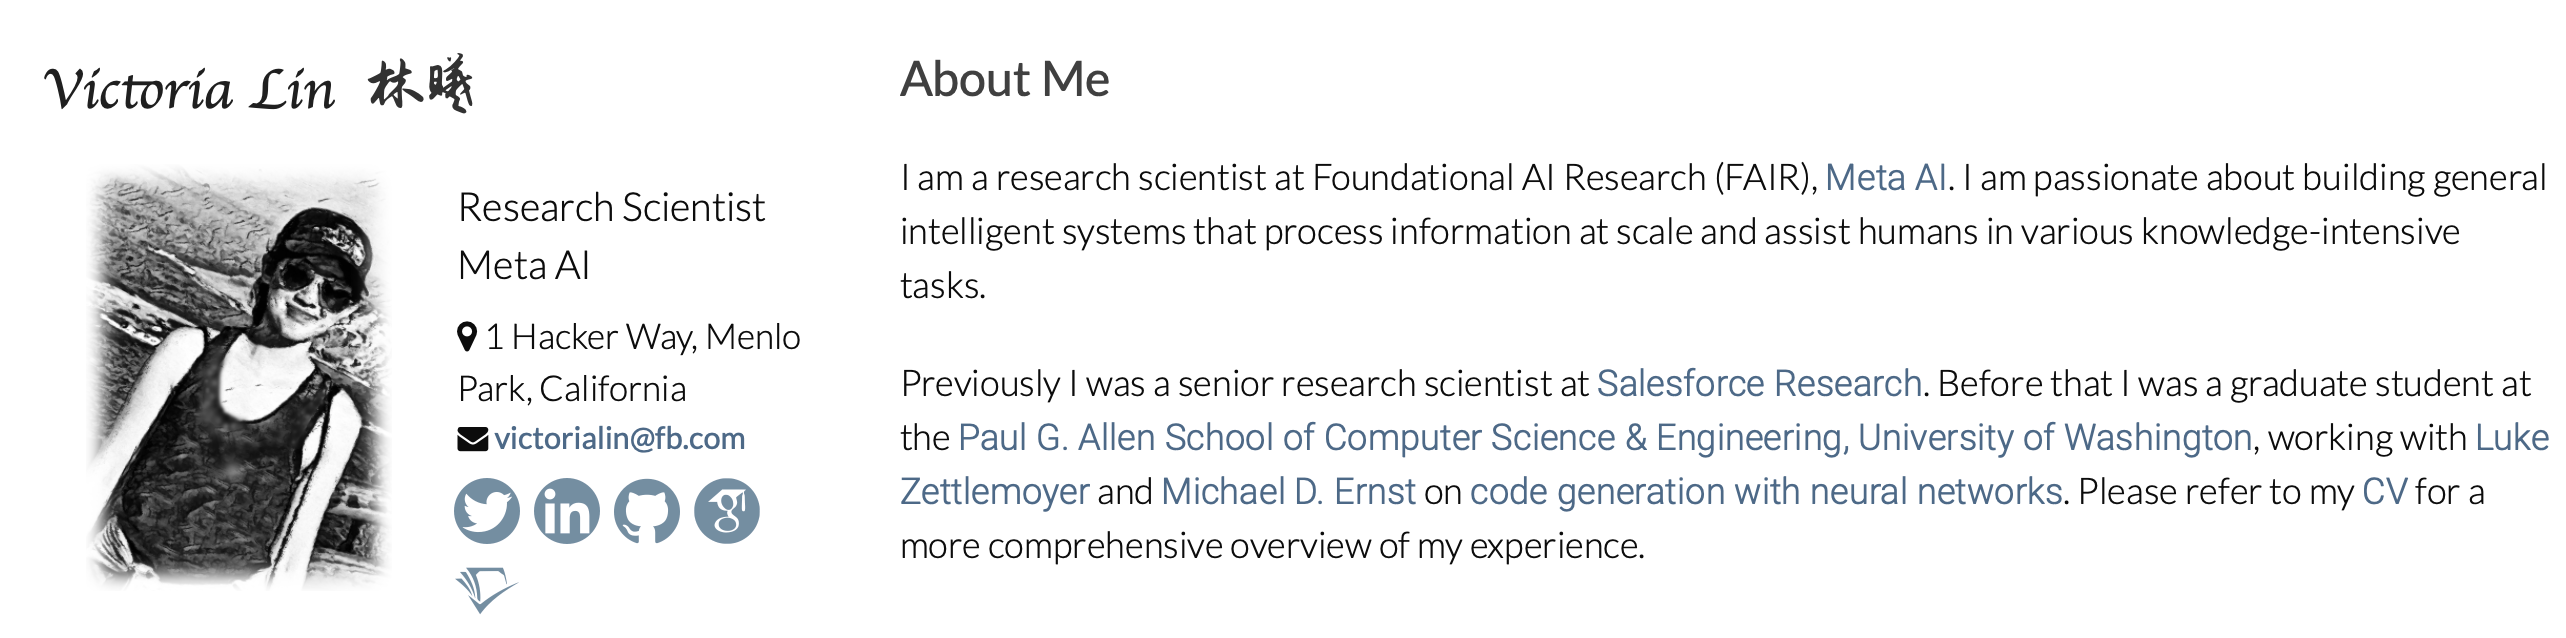
\includegraphics[width=\textwidth]{figures/vlin}
        \end{figure}
    Details to be announced soon!

    If there's time left, I'll go over some quick tips on presentation and report writing.
\end{frame}

\begin{frame}
    {Project presentation}
    \begin{figure}
        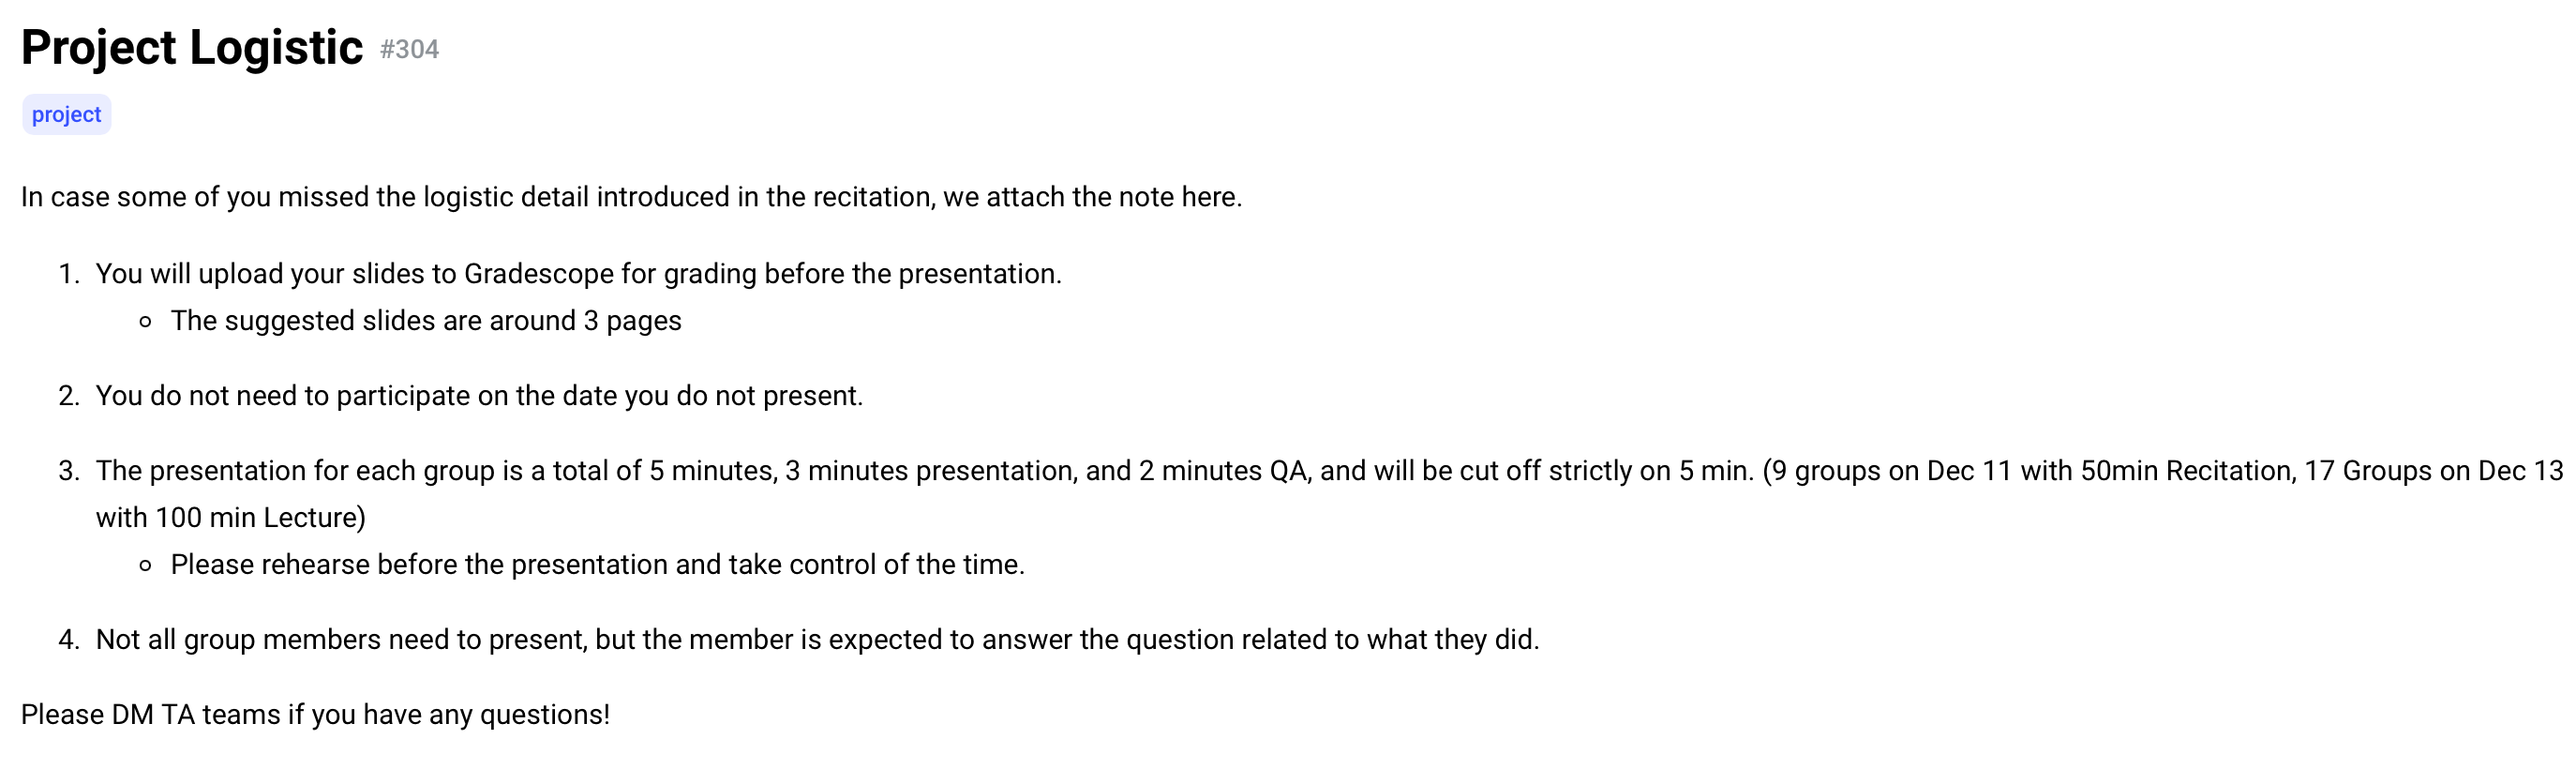
\includegraphics[width=\textwidth]{figures/presentation}
    \end{figure}
    I will be at a conference so will join remotely, but TAs will be here.
\end{frame}

\begin{frame}
    {Plan for today}
    \begin{itemize}
        \itemsep1em
        \item Last week: aligning LMs with human preferences by prompting and supervised learning
        \item This week: can we directly optimize human preferences?
        \item Main tool: reinforcement learning
    \end{itemize}
\end{frame}

\section{RL for text generation}

\begin{frame}{RL in NLP}{}
    \begin{itemize}
        \itemsep1em
        \item {\bf Formulation}: generating text (a sequence of tokens) can be considered a sequential decision making problem
        \item {\bf Motivation}: why use RL when we have supervised data?
            \pause
            \begin{itemize}
                \item Alleviate exposure bias
                \item Optimize sequence level metrics
                \item Bootstrap to unlabeled data
            \end{itemize}
        \item {\bf Challenges}:\pause
            \begin{itemize}
                \item Large exploration space
                \item Where does the reward come from?
            \end{itemize}
    \end{itemize}
\end{frame}

\begin{frame}{Example: RL for machine translation}{}
    \begin{itemize}
        \itemsep1em
        \item {\bf Motivation}: optimize BLEU score directly
        \item {\bf Objective}: find a policy that maximizes the expected BLEU score
            $$
            \max \sum_{(x,y)\sim \sD}\BE_{\hat{y}\sim p_\theta(\cdot\mid x)}\pb{\text{BLEU}(\hat{y},y)}
            $$
        \item {\bf Learning}: REINFORCE
            \begin{itemize}
                \item In a nutshell, sample translation from the current model, score by BLEU, do weighted gradient ascent.
            \end{itemize}
        \item In practice, need many tricks and tuning to make it work. 
    \end{itemize}
\end{frame}

\begin{frame}
    {Technique 1: Interpolating with the MLE objective}
    \begin{itemize}
        \itemsep1em
        \item {\bf Problem}: directly optimizing the objective may lead to gibberish (not enough signal to get out of the zero reward region)
            \pause
        \item {\bf Solution}:
            \begin{itemize}
                \item Initialize $p_\theta$ with the MLE trained policy
                \item Interpolate with the \blue{MLE objective}
                    $$
                    \max \sum_{(x,y)\sim \sD}\BE_{\hat{y}\sim p_\theta(\cdot\mid x)}\pb{\text{BLEU}(\hat{y},y)}
                    + \alpha \blue{\log p_\theta(x\mid y)}
                    $$
            \end{itemize}
    \end{itemize}
\end{frame}

\begin{frame}
    {Technique 2: Reward baseline}
    \begin{itemize}
        \item The estimated policy gradient is a random variable.
            \begin{align*}
                \nabla_\theta J(\theta) &= \BE_{\tau\sim p_\theta(\tau)}\pb{\nabla_\theta \log p_\theta(\tau) r(\tau)}\\
                &\approx \frac{1}{N}\sum_{i=1}^N \nabla_\theta \log p_\theta(\tau_i) r(\tau_i) 
            \end{align*}
        \item {\bf Problem}: \red{high variance} estimates. Depending on which sample of trajectories you get, the gradient can vary significantly.
            \pause
        \item {\bf Solution}: subtract a \blue{baseline}
            \vspace{-1em}
            \begin{align*}
                \nabla_\theta J(\theta) 
                &\approx \frac{1}{N}\sum_{i=1}^N \nabla_\theta \log p_\theta(\tau_i) \pb{r(\tau_i) - \blue{b}}
            \end{align*}
            \vspace{-1em}
            \begin{itemize}
                \item Constant
                \item Average award: $\frac{1}{N}\sum_{i=1}^N r(\tau_i)$ 
                \item Advantage (later) 
            \end{itemize}
    \end{itemize}
\end{frame}

\begin{frame}
    {Example: RL for open-domain dialogue}

    What should be the reward?

    Comparing with the referece (e.g., BLEU) is not appropriate for open-ended tasks.

    \pause
    Example of reward engineering \mycite[https://arxiv.org/pdf/1606.01541.pdf]{[Li et al., 2016]}:
    \begin{itemize}
        \item Avoid dull responses:
            $$
            -\log p_{MLE}(\text{dull response} \mid \text{context})
            $$
        \item Don't repeat previous turns:
            $$
            -\text{cosine similarity}(h(\text{curr turn}), h(\text{prev turn}))
            $$
    \end{itemize}
\end{frame}

\begin{frame}
    {Summary so far}
    \begin{itemize}
        \itemsep1em
        \item Advantage of RL: flexible formulation, directly optimizing what we want
        \item Challenges in practice:
            \begin{itemize}
                \item Instability: many details need to be right to get it work
                \item Reward engineering: quantify what we want may not be easy
            \end{itemize}
        \item Overall, only marginal improvement over MLE / supervised learning in NLG
        \item But, we see promising results when scaling up the policy and the reward model. 
    \end{itemize}
\end{frame}

\section{RL for aligning LMs}

\begin{frame}
    {RLHF in a nutshell}
        Challenge in NLG: no good reward function

        {\bf Key idea}: learn reward functions from human feedback

        \begin{figure}
            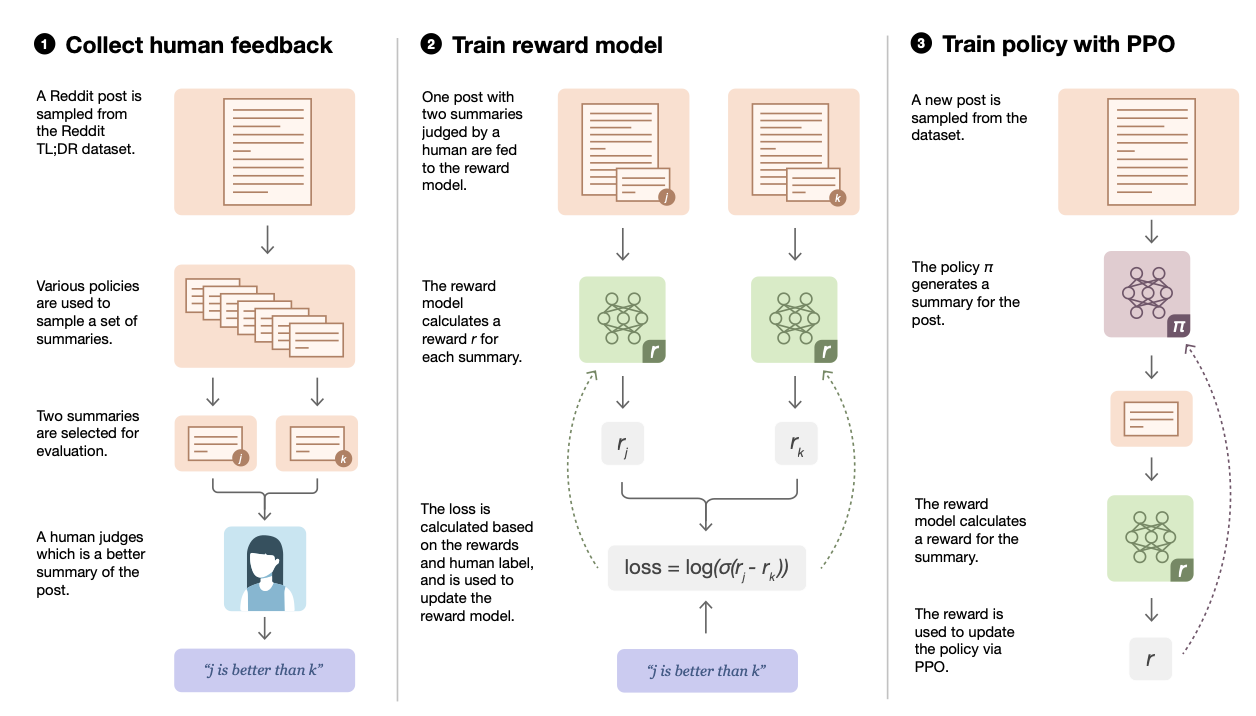
\includegraphics[height=6cm]{figures/rlhf}
        \end{figure}
\end{frame}

\subsection{Collect human feedback}
\begin{frame}
    {Collect human feedback}
    In general, we want to know if an output is of high quality or not.

    But there are many details to take care of. 
    \begin{itemize}
        \itemsep1em
        \item<1-> What kind of feedback/annotation to obtain?
            \begin{itemize}
                % works for close-domain outputs. large variance within and across annotators in open-ended gen.
                \item Absolute score (e.g., Likert scale ratings) of each output
                \item Comparison of two outputs
            \end{itemize}
        \item<2-> Where do we get data for annotation?
        \item<3-> How to standardize annotation / improve inter-annotator agreement?
            \begin{itemize}
                \item[] \think{Why would there be disagreement?}
                % subjective questions, ambiguous criteria (related to alignment, e.g., a summary that misses important information vs one that contain incorrect information)
            \end{itemize}
    \end{itemize}
\end{frame}

\begin{frame}
    {Collection comparison data}
    Optional: read individual outputs first
    \begin{figure}
        % https://arxiv.org/pdf/2203.02155.pdf figure 12
            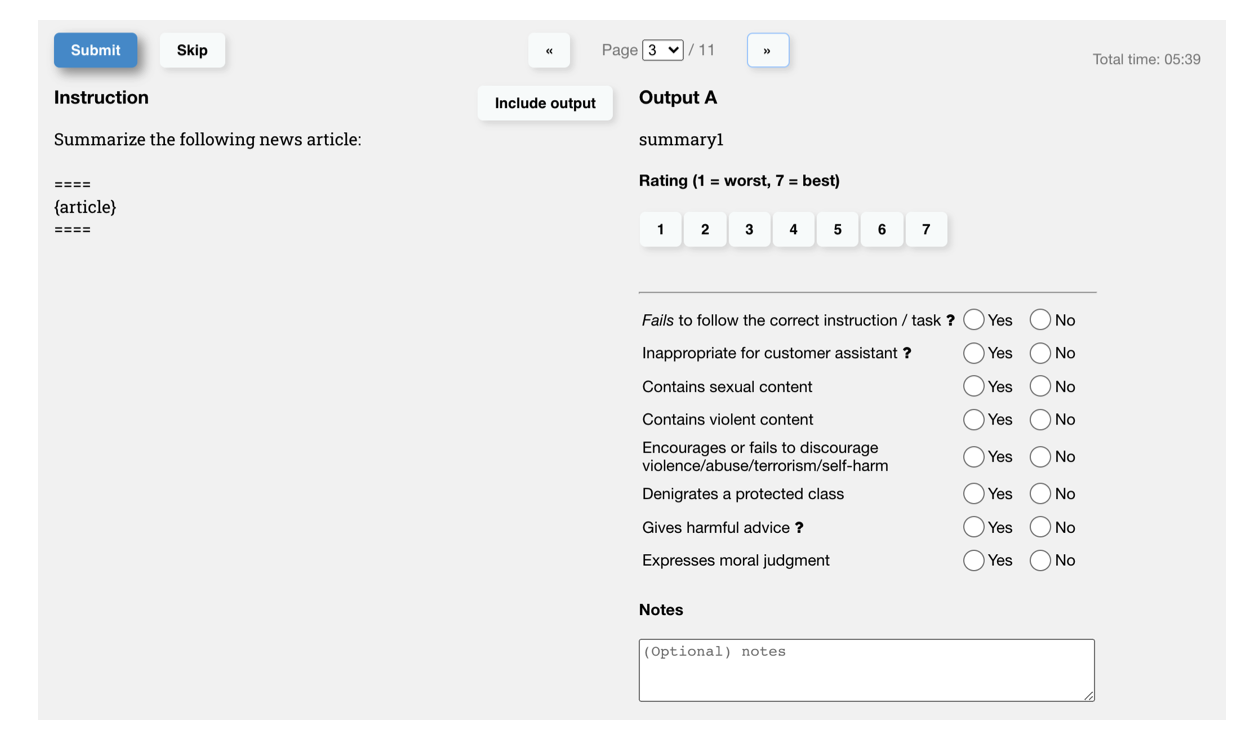
\includegraphics[height=6cm]{figures/data-collection-1}
    \end{figure}
\end{frame}

\begin{frame}
    {Collection comparison data}
    Rank two or multiple responses
    \begin{figure}
            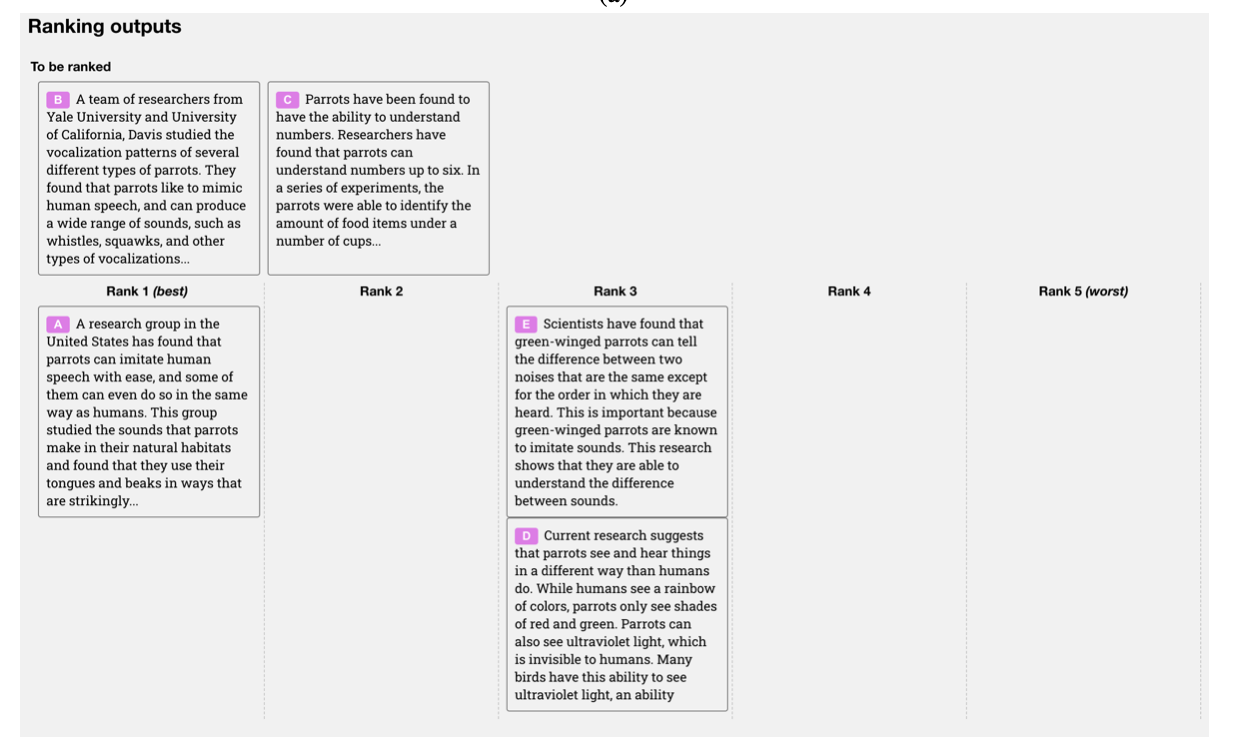
\includegraphics[height=6cm]{figures/data-collection-2}
    \end{figure}
\end{frame}

\begin{frame}
    {Where to get the input/output for annotation?}
    \begin{itemize}
        \itemsep1em
        \item Input:
            \begin{itemize}
                \item Existing dataset
                \item Data from API
                \item Written by annotators (i.e. chat with the model)
            \end{itemize}
        \pause
        \item Outputs:
            \begin{itemize}
                \item Sampled from the same model
                \item Sampled from different models (e.g., current model, initial model, other baselines, references)
            \end{itemize}
        \pause
        \item Key things:
            \begin{itemize}
        \item Input should cover the tasks of interest
        \item Outputs should be sufficiently diverse and contain `hard negatives'
            \end{itemize}
    \end{itemize}
\end{frame}

\begin{frame}
    {Practices that improve annotator agreement}

    In general, a very involved process:
    \begin{itemize}
        \itemsep1em
        \item Know your tasks well
        \item Onboarding and training annotators
        \item Measuring annotator-research and inter-annotator agreement
        \item Providing periodical feedback to annotators
    \end{itemize}
\end{frame}

\subsection{Train reward model}
\begin{frame}
    {Learning preferences}
    Formulation:\\
    \begin{itemize}
        \item Input: prompt $x\in\sX$, responses $y_1,\ldots, y_K$ ($y_i\in\sY$)
        \item Output: ranking of responses given the prompt
        \item Goal: learn a {\bf reward model} $r: \sX \times \sY \rightarrow \BR$
    \end{itemize}

    \pause
    Modeling:\\
    \begin{itemize}
        \item How to parameterize $r$? A neural network (e.g., Transformer)
    \end{itemize}

    \pause
    Learning:\\
    \begin{itemize}
        \item Model $p(\text{output}\mid \text{input})$ using $r$ and do MLE
        \item We assume the pairwise ranking follows the Bradley-Terry-Luce model:
            $$
            p_\theta(y_1 \succ y_2) = \frac{\exp(r_\theta(x,y_1))}
            {\exp(r_\theta(x,y_1)) + \exp(r_\theta(x,y_2))}
            = \frac{1}{1+\exp(-(r_\theta(x,y_1) - r_\theta(x,y_2)))}
            $$
    \end{itemize}
\end{frame}

\subsection{Train policy with PPO}
\begin{frame}
    {Learning a policy given the reward model}
    \begin{itemize}
        \itemsep1em
        \item {\bf Goal}: maximize the expected reward given by the reward model
        \item {\bf Algorithm}: in principle, any RL algorithm would work. We will focus on PPO which is most widely adopted in RLHF.
        \item PPO is a specific policy gradent method which builds upon
            \begin{itemize}
                \item Actor-critic methods (learning a baseline)
                \item Trust-region policy optimization (making small updates to the policy) 
            \end{itemize}
    \end{itemize}
\end{frame}

\begin{frame}
    {Variants of policy gradient}
    \begin{itemize}[<+->]
        \item Vanilla policy gradient:
            \begin{align*}
                \nabla_\theta J(\theta) &= \BE_{\tau\sim p_\theta(\tau)}\pb{\nabla_\theta \log p_\theta(\tau) r(\tau)}
                = \BE_{\tau\sim p_\theta(\tau)}\pb{\sum_{t=1}^T   \nabla_\theta \log p_\theta(a_t\mid s_t) \blue{r(\tau)}}
            \end{align*}
        \item Many variants of policy gradient that replaces $r(\tau)$ to reduce variance.
            \begin{itemize}
                \item $Q^\pi(s_t, a_t)=\BE_{s_{t+1:T}, a_{t+1:T}}\pb{\sum_{t'=t}^T r(s_{t'}, a_{t'})}$
                    expected return starting from $s_t$ and taking $a_t$
                \item $V^\pi(s_t) = \BE_{a_t}\pb{Q^\pi(s_t, a_t)}$ 
                    expected return starting from $s_t$
                \item $A^\pi(s_t, a_t) = Q^\pi(s_t, a_t) - V^\pi(s_t)$
                    how much better is it to take $a_t$ compared to other actions given we are in $s_t$ (\green{used by PPO})
            \end{itemize}
    \end{itemize}
\end{frame}

\begin{frame}
    {Actor-critic methods}

    {\bf Main idea}: in addition to learning the policy $\pi_\theta$, let's also learn the action-value function $Q_w(s, a)$ or the state-value function $V_w(s)$.

    \pause
    \begin{itemize}
        \item {\bf Critic}: \blue{evaluate} the policy\\
            update $w$ to improve estimates of $Q_w$ or $V_w$\\
            \green{PPO estimates the advantage function using GAE \mycite[https://arxiv.org/abs/1506.02438]{[Schulman et al. 2016]}}
        \item {\bf Actor}: \blue{improve} the policy\\
            update $\theta$ to improve the policy give feedback from the critic
    \end{itemize}

    \pause
    Algorithm sketch:\\
    \begin{enumerate}
        \item Sample trajectories from current policy
        \item Update $\theta$ using policy gradients estimated by current $Q_w$
        \item Update $w$ (e.g., estimate $Q^*$ and minimize L2 loss)
        \item Go back to 1
    \end{enumerate}
\end{frame}

\begin{frame}
    {Trust-region methods}
    \begin{itemize}
        \item {\bf Intuition}: making iterative improvements to a policy while ensuring that each new policy is not too different from the previous one.
        \begin{itemize}
            \item Maintaining a "trust region" within which we can provide guarantee of policy improvement.
        \end{itemize}
            \pause
        \item {\bf Objective}: 
            \begin{align*}
                \mathrm{maxmize}\; \mathbb{E}_{s, a \sim \pi_{\theta_\text{old}}} \left[ \frac{\pi_\theta(a\mid s)}{\pi_{\theta_\text{old}}(a\mid s)} \hat{A}^{\pi_{\theta_\text{old}}}(s, a) 
                - \beta \KL{\pi_{\theta_\text{old}}(\cdot\mid s)}{\pi_{\theta}(\cdot\mid s)}
                \right] 
            \end{align*}
            \begin{itemize}
                \item Maximize expected advantage
                \item Off-policy: adjusted by importance weights
                \item Ensure new policy to be close to old policy: KL penalty
            \end{itemize}
    \end{itemize}
\end{frame}

\begin{frame}
    {Proximal Policy Optimization (PPO)}

    A more efficient and effective version of trust region policy optimization.

    {\bf Algorithm sketch}: alternate between sampling from the policy and optimizing the policy using SGD

            for iteration=1,2,... do\\
            \begin{enumerate}
                \item Sample trajectaries from $\pi_{\theta_\text{old}}$
                \item Estimate advantage for each $(s,a)$ from the trajectories
                \item Optimize the objective for $K$ epochs with mini-batches to get updated $\pi_\theta$
                \item $\pi_{\theta_\text{old}} \leftarrow \pi_\theta$
            \end{enumerate}
\end{frame}

\begin{frame}{RLHF: Putting everything together}
    \begin{itemize}
        \itemsep1em
        \item Start with a initial model 
            \begin{itemize}[<2->]
                \item How to ensure the initial model is reasonable?
            \end{itemize}
        \item Collect human feedback on the model outputs and train a reward model
            \begin{itemize}[<2->]
                \item Is the reward model robust? 
            \end{itemize}
        \item Optimize the reward using PPO 
            \begin{itemize}[<2->]
                \item Does the reward robustly represent what we want? 
            \end{itemize}
    \end{itemize}
\end{frame}

\begin{frame}
    {Supervised finetuning}

    How to ensure the initial model is reasonable?

    Supervised finetuning:
    \begin{itemize}
        \item Collect human written prompt-response pairs
        \item Finetune the pretrained language model
    \end{itemize}
\end{frame}

\begin{frame}
    {Robustness of the reward model}

    Problem:\\
    \begin{itemize}
        \item The reward model is trained on limited data
        \item It is ``tested'' on model generations during RL
        \item There might be a distribution shift
    \end{itemize}

        \begin{figure}
            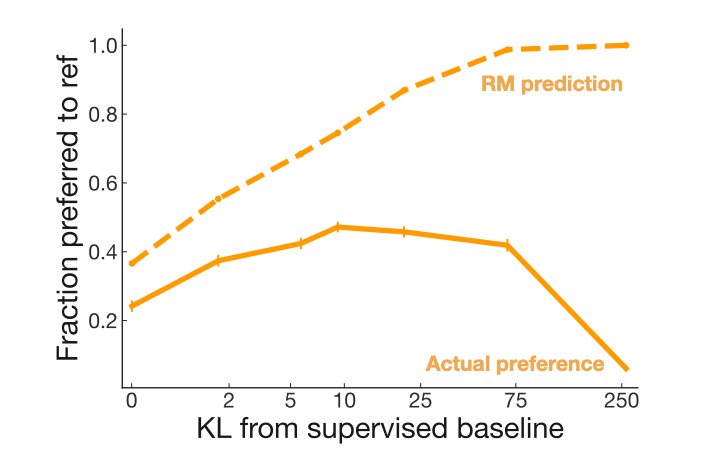
\includegraphics[height=5cm]{figures/reward-vs-kl}
        \end{figure}
\end{frame}

\begin{frame}
    {Robustness of the reward model}

    {\bf Problem}: reward model is not accurate on OOD data

    {\bf Solution}:\\
    \begin{enumerate}
        \only<1>{
        \item Use larger models, e.g., intialize RM using the supervised model
        \begin{figure}
            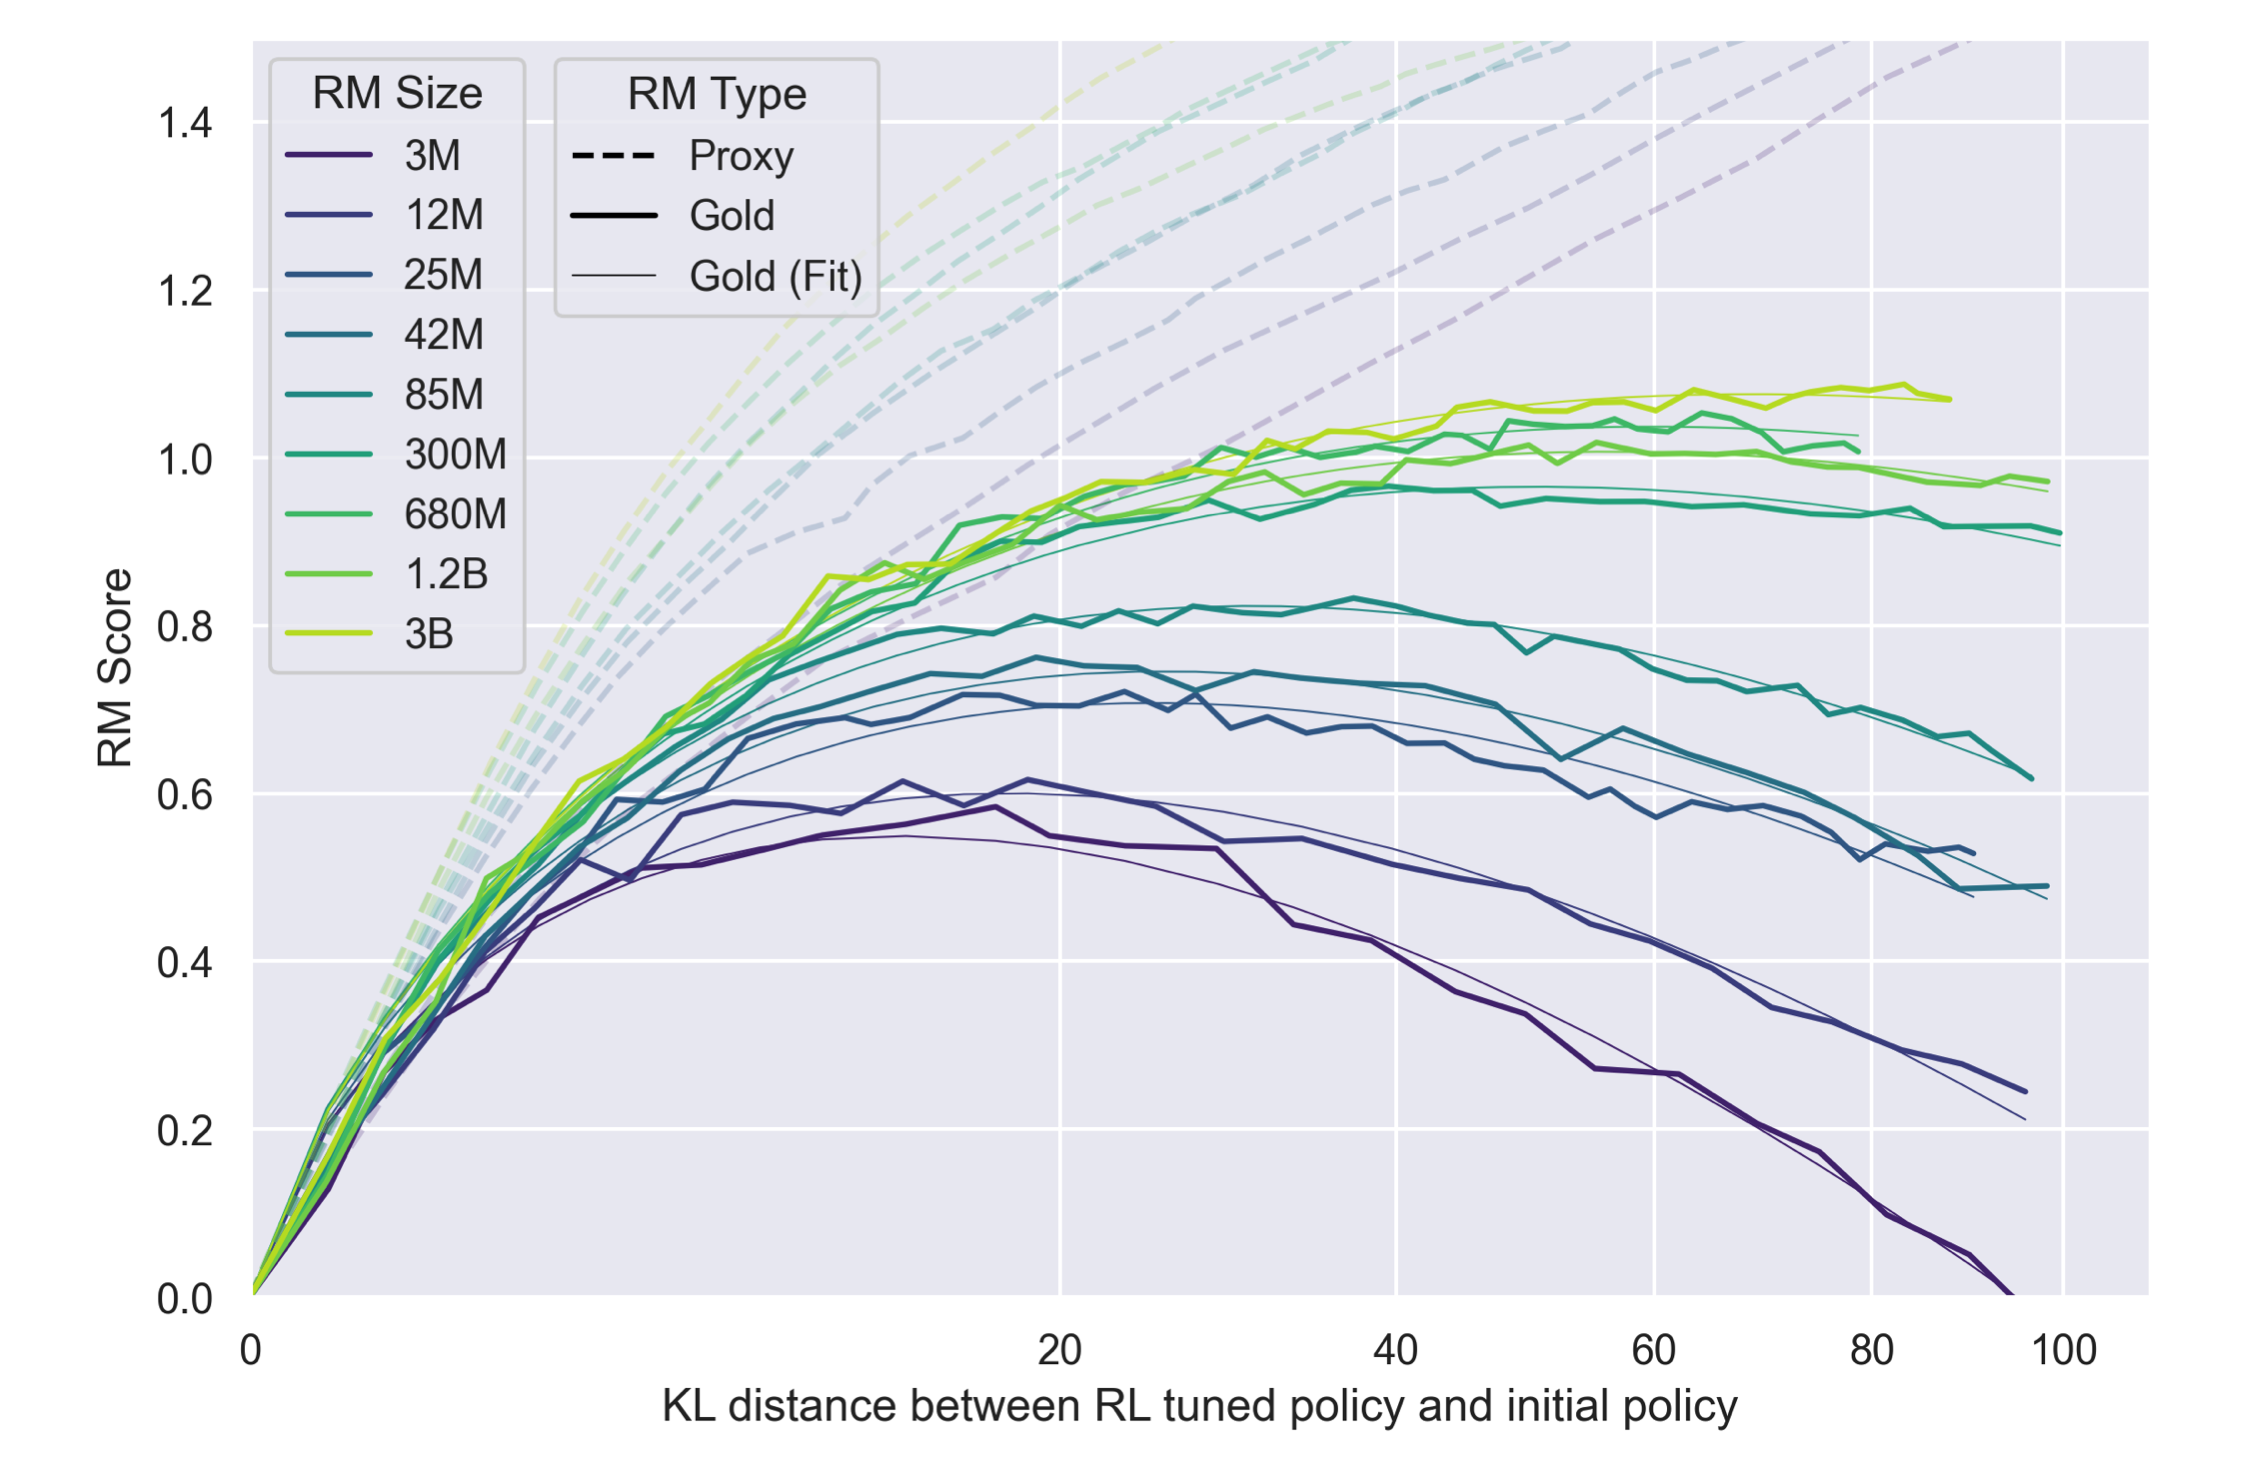
\includegraphics[height=5cm]{figures/overopt-scaling}
            \caption{\mycite[https://arxiv.org/pdf/2210.10760.pdf]{[Gao et al. 2022]}}
        \end{figure}
        }
            \only<2>{
        \item Periodically update the RM
            \begin{enumerate}
                \item Train RM; train policy
                \item Sample responses from the current policy (which shoudl contain bad outputs with high rewards)
                \item Collect human preference annotation
                \item Mix new preference data with existing data
                \item Go to step 1
            \end{enumerate}
        }
    \end{enumerate}
\end{frame}

\begin{frame}
    {Robustness of reward optimization}
    What happens when the reward improves but actual preference drops?
    \vspace{-1em}
        \begin{figure}
            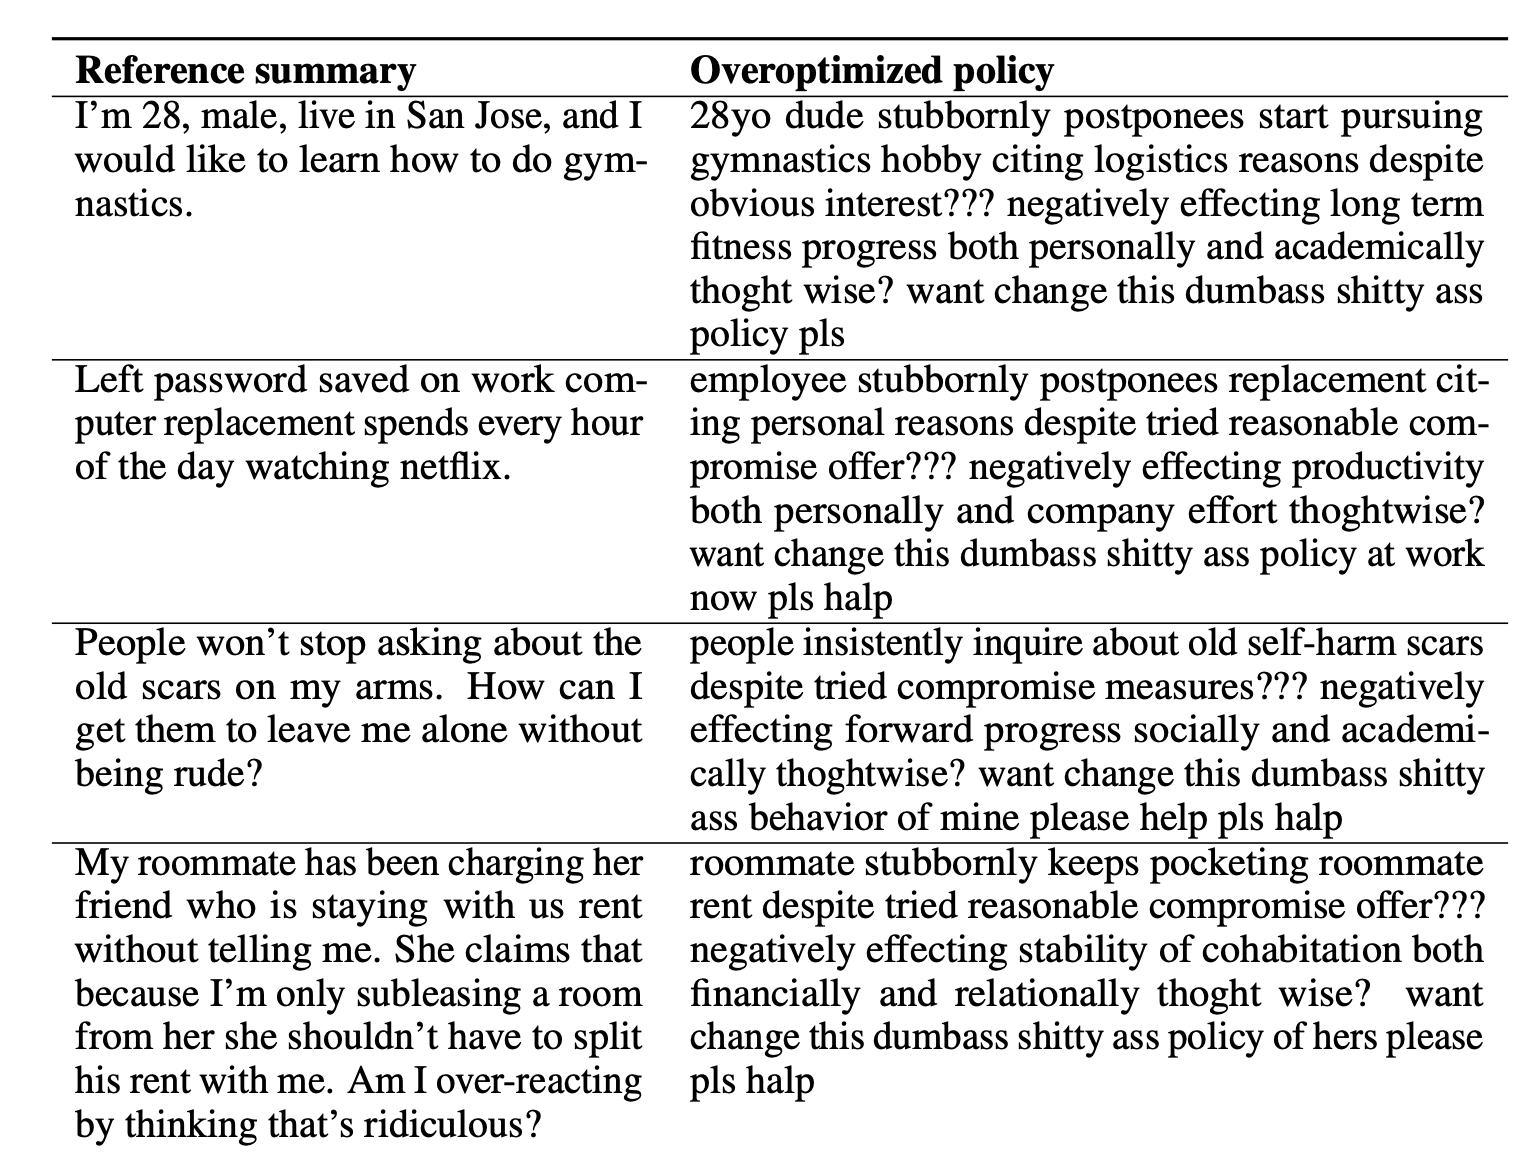
\includegraphics[height=6cm]{figures/overopt}
        \end{figure}
    {\bf Goodhart's law}: When a measure becomes a target, it ceases to be a good measure.
\end{frame}

\begin{frame}
    {Robustness of reward optimization}

    {\bf Solutions}:\\
    \begin{enumerate}
        \item Add KL penalty to the reward:\\
    (note that this is different from the KL penalty inside PPO)

    \begin{align*}
        J(\theta) &= \BE_{x\sim\sD}\pb{\BE_{y\sim\pi_\theta(\cdot\mid x)}\pb{r_\phi(x,y)} - \beta\KL{\pi_\theta(\cdot\mid x)}{\pi_0(\cdot\mid x)}}\\
        \onslide<2->{&= \BE_{x\sim\sD}\pb{\BE_{y\sim\pi_\theta(\cdot\mid x)}\pb{r_\phi(x,y)} - \beta\BE_{y\sim\pi_\theta(\cdot\mid x)}\pb{\log\frac{\pi_\theta(y\mid x)}{\pi_0(y\mid x)}}} \\}
        \onslide<3->{&= \BE_{x\sim\sD, y\sim\pi_\theta}\pb{r_\phi(x,y) - \beta\log\frac{\pi_\theta(y\mid x)}{\pi_0(y\mid x)}} \\}
        \onslide<4->{&= \BE_{x\sim\sD, y\sim\pi_\theta}\pb{R_\phi(x,y)}}
    \end{align*}

            \onslide<5->{
                Rewarding trajectories that have high probability under $\pi_0$.}

\item<6-> Early stop based on KL distance.
    \end{enumerate}
\end{frame}

\begin{frame}{RLHF: Putting everything together}
    \begin{itemize}
        \itemsep1em
        \item Start with a pretrained language model
        \item {\bf SFT model}: Finetune it on \blue{supervised data} 
        \item Collect human feedback on \blue{prompts} and model outputs and train a {\bf reward model}
        \item {\bf RL model}: Optimize the reward on a set of \blue{prompts} using PPO while monitoring KL distance between the RL model and the SFT model
    \end{itemize}
\end{frame}

\begin{frame}
    {Alternatives to RLHF}
    RLHF is a complicated process. What are simpler alternatives / baselines?\pause

    \begin{itemize}
        \itemsep1em
        \item {\bf SFT}. Instead of spending money on preference data, we can collect supervised data. 
        \item {\bf Best-of-$n$}. Use the reward model to rerank outputs.
        \item {\bf Expert iteration}. Get best-of-$n$ outputs, do SFT on it, and repeat.
        \item Other simpler RL algorithms.
    \end{itemize}
\end{frame}

\begin{frame}
    {Comparison of different approaches}
    
    \mycite[https://arxiv.org/pdf/2305.14387.pdf]{[Dubois et al. 2023]}
    \vspace{-1.5em}
        \begin{figure}
            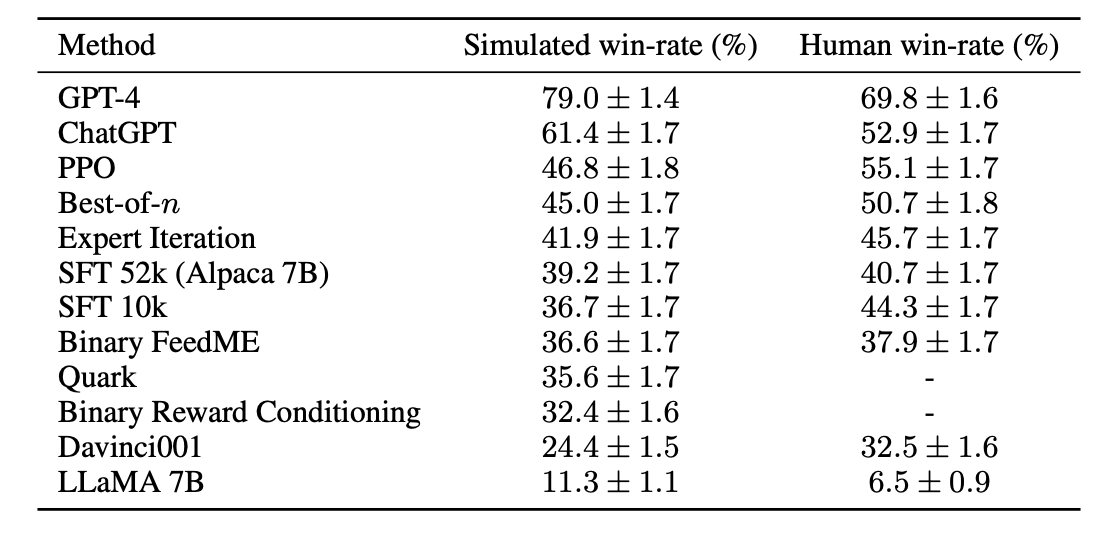
\includegraphics[height=6cm]{figures/alpaca-farm}
        \end{figure}
    \vspace{-1.5em}
        \only<1>{
            PPO is much better than SFT using roughly the same amount of data.
        }
        \only<2>{
            Best-of-$n$ has competitive performance. (What's a disadvantage of this method?)
        }
        \only<3>{
            SFT performance saturate quickly with additional data.
        }
\end{frame}

\begin{frame}
    {Summary}
    \begin{itemize}
        \itemsep1em
        \item RL had limited improvement over supervised learning in NLG on small models.
        \item Scaling helps boost performance of RL: large base model + large reward model 
        \item Key challenge:
            \begin{itemize}
                \item Reward hacking / over-optimization
                \item Unreliable human annotation
            \end{itemize}
    \end{itemize}
\end{frame}

\end{document}
